\documentclass[12pt]{article}

%useful packages
\usepackage{color,soul}
\usepackage[usenames,dvipsnames,svgnames,table]{xcolor}
\usepackage{amsmath,amsthm,amscd,amssymb,bm}
\usepackage{hyperref}
\hypersetup{
    colorlinks=true,
    linkcolor=JungleGreen
}
\usepackage[utf8]{inputenc}
\usepackage[top=2cm, bottom=3cm, left=2cm, right=2cm]{geometry}
\usepackage{pgfplots}
\usepackage{enumitem}
\usepgfplotslibrary{fillbetween}
\usetikzlibrary{patterns}
\usepackage{tcolorbox}
\usepackage{centernot}
\usepackage{mathtools}
\usepackage{xcolor}

%personal definitions and commands
\newcommand{\R}{\mathbb{R}} 
\newcommand{\E}{\mathbb{E}}
\newcommand{\V}{\mathbb{V}}
\newcommand{\C}{\mathbb{C}}
\newcommand{\Prob}{\mathbb{P}}
\newcommand{\e}{\epsilon}
\newcommand\numberthis{\addtocounter{equation}{1}\tag{\theequation}} %allows numbering of single equations in align* environment
\newcommand{\mtx}[1]{\ensuremath{\bm{\mathit{#1}}}}
\newcommand{\B}{\hat{\boldsymbol{\beta}}}
\newcommand{\Cov}{\mathbb{C}\text{ov}}
\newcommand{\N}{\mathcal{N}}



\title{ECON675: Assignment 2}
\author{Anirudh Yadav\thanks{I worked on the code for this assignment with several classmates.}}
\setlength\parindent{0pt}
\begin{document}

\maketitle
\setcounter{tocdepth}{2}
\tableofcontents

\newpage

\section{Kernel density estimation}

\subsection{Density derivatives}
I follow the derivation in Hansen's notes. We are interested in estimating
\begin{align*}
f^{(s)}(x) = \frac{d^s}{dx^s}f(x).
\end{align*}
The natural estimator is
\begin{align*}
\hat f^{(s)}(x)= \frac{d^s}{dx^s}\hat f(x)
\end{align*}
Now, we know that $\hat f(x) = \frac{1}{nh}\sum_i K\left(\frac{X_i - x}{h}\right)$. Thus,
\begin{align*}
\hat f^{(1)}(x) &= \frac{-1}{nh^2}\sum_{i=1}^n K^{(1)}\left(\frac{X_i - x}{h}\right),\\
\hat f^{(2)}(x) &= \frac{1}{nh^3}\sum_{i=1}^n K^{(2)}\left(\frac{X_i - x}{h}\right),\\
&\vdots \\
\hat f^{(s)}(x) &= \frac{(-1)^s}{nh^{1+s}}\sum_{i=1}^n K^{(s)}\left(\frac{X_i - x}{h}\right).
\end{align*}
Now,
\begin{align*}
\E[\hat f^{(s)}(x)] &= \frac{1}{n} \sum_{i=1}^n \E\left[ \frac{(-1)^s}{h^{1+s}}K^{(s)}\left(\frac{X_i - x}{h}\right)\right]\\
&=\E\left[ \frac{(-1)^s}{h^{1+s}}K^{(s)}\left(\frac{X_i - x}{h}\right)\right], \text{ since $X_i$ are iid}.\\
&=\int_{-\infty}^{\infty} \frac{(-1)^s}{h^{1+s}}K^{(s)}\left(\frac{z - x}{h}\right)f(z)dz
\end{align*}
Next, we want to use integration by parts: $\int u dv = uv - \int vdu$. Define
\begin{align*}
dv = \frac{(-1)^s}{h^{s}}\frac{1}{h}K^{(s)}\left(\frac{z - x}{h}\right) \implies v = \frac{(-1)^s}{h^{s}}K^{(s-1)}\left(\frac{z - x}{h}\right)
\end{align*}
And
\begin{align*}
u = f(z) \implies du = f^{(1)}(z).
\end{align*}
Thus,
\begin{align*}
\E[\hat f^{(s)}(x)] &= \left[ \frac{(-1)^s}{h^{s}}K^{(s-1)}\left(\frac{z - x}{h}\right)  f^{(1)}(z)\right]_{-\infty}^{\infty} - \int_{-\infty}^\infty \frac{(-1)^s}{h^{s}}K^{(s-1)}\left(\frac{z - x}{h}\right) f^{(1)}(z)dz.\\
&=- \int_{-\infty}^\infty \frac{(-1)^s}{h^{s}}K^{(s-1)}\left(\frac{z - x}{h}\right) f^{(1)}(z)dz
\end{align*}
Repeating this $s$ times give
\begin{align*}
\E[\hat f^{(s)}(x)] &= (-1)^s \int_{-\infty}^\infty \frac{(-1)^s}{h}K\left(\frac{z - x}{h}\right) f^{(s)}(z)dz\\
&=\int_{-\infty}^\infty \frac{1}{h}K\left(\frac{z - x}{h}\right) f^{(s)}(z)dz
\end{align*}
Next, use the following change of variables: $u = \frac{z - x}{h}$, which implies $z = x + hu \implies dz = hdu$, to get
\begin{align}
\E[\hat f^{(s)}(x)] &= \int_{-\infty}^\infty K(u) f^{(s)}(x+hu)du \label{eq:der1}
\end{align}
The next step is to take a Taylor expansion of $f^{(s)}(x+hu)$ around $x+hu = x$, which is valid if $h \to 0$. We get
\begin{align*}
f^{(s)}(x+hu) = f^{(s)}(x) + f^{(s+1)}(x)hu + \frac{1}{2}f^{(s+2)}(x)h^2u^2 + ... + \frac{1}{P!} f^{(s+P)}(x)h^Pu^P + o(h^P).
\end{align*}
Substituting this expression back into (\ref{eq:der1}), integrating over each term, and using the fact that $\int_{-\infty}^\infty K(u)du = 1$ and the notation
\begin{align*}
\mu_\ell(K) = \int u^\ell K(u) du
\end{align*}
gives
\begin{align*}
\E[\hat f^{(s)}(x)] &= f^{(s)}(x) + f^{(s+1)}(x)h\mu_1(K) + \frac{1}{2}f^{(s+2)}(x)h^2\mu_2(K) + ... + \frac{1}{P!} f^{(s+P)}(x)h^P\mu_P(K) + o(h^P).
\end{align*}
Finally, noting that since $K$ is a $P$-order kernel, $\mu_\ell(K) = 0$ for all $\ell < P$, gives the desired result
\begin{align}
\E[\hat f^{(s)}(x)] &= f^{(s)}(x) + \frac{1}{P!} f^{(s+P)}(x)h^P\mu_P(K) + o(h^P). \label{eq:der2}
\end{align}

Next we consider the variance of the derivative estimator.
\begin{align*}
\V[\hat f^{(s)}(x)] &= \V\left[\frac{(-1)^s}{nh^{1+s}}\sum_{i=1}^n K^{(s)}\left(\frac{X_i - x}{h}\right)\right]\\
&=\frac{1}{nh^{2+2s}}\V\left[K^{(s)}\left(\frac{X_i - x}{h}\right)\right],
\end{align*}
since $\{X_i\}$ are iid there are no covariance terms and each term has the same variance. Continuing,
\begin{align}
\V[\hat f^{(s)}(x)] &=\frac{1}{nh^{2+2s}} \left\{\E\left[K^{(s)}\left(\frac{X_i - x}{h}\right)^2\right] - \E\left[K^{(s)}\left(\frac{X_i - x}{h}\right)\right]^2 \right\} \nonumber \\
&=\frac{1}{nh^{2+2s}} \E\left[K^{(s)}\left(\frac{X_i - x}{h}\right)^2\right] - \frac{1}{n} \E\left[\frac{1}{h^{1+s}}K^{(s)}\left(\frac{X_i - x}{h}\right)\right]^2 \label{eq:der3}
\end{align}
Now, from above we know that
\begin{align*}
\E\left[\frac{1}{h^{1+s}}K^{(s)}\left(\frac{X_i - x}{h}\right)\right] & =  f^{(s)}(x) + \frac{1}{P!} f^{(s+P)}(x)h^P\mu_P(K) + o(h^P)\\
&= f^{(s)}(x) + o(1)
\end{align*}
since the remainder goes to zero as $h\to0$. Thus, the second term in (\ref{eq:der3}) is $O(\frac{1}{n})$; i.e. the same order as $1/n$. Furthermore $O(\frac{1}{n})$ is of smaller order than $O(\frac{1}{nh^{1+2s}})$ since $h \to 0$ and $n\to \infty$. Accordingly, we can write
\begin{align*}
\V[\hat f^{(s)}(x)] &=\frac{1}{nh^{2+2s}} \E\left[K^{(s)}\left(\frac{X_i - x}{h}\right)^2\right] + o\left(\frac{1}{nh^{1+2s}}\right),
\end{align*}
Thus,
\begin{align*}
\V[\hat f^{(s)}(x)] &=\frac{1}{nh^{1+2s}} \int_{-\infty}^{\infty}\frac{1}{h}K^{(s)}\left(\frac{z- x}{h}\right)^2 f(z) dz + o\left(\frac{1}{nh^{1+2s}}\right)
\end{align*}
Again we use the change of variables $u = \frac{z - x}{h}$ so that
\begin{align*}
\V[\hat f^{(s)}(x)] &=\frac{1}{nh^{1+2s}} \int_{-\infty}^{\infty}K^{(s)}(u)^2 f(x+hu) du + o\left(\frac{1}{nh^{1+2s}}\right)
\end{align*}
With the usual Taylor expansion of $f(x+hu)$ we can write
\begin{align*}
\V[\hat f^{(s)}(x)] &=\frac{1}{nh^{1+2s}} \int_{-\infty}^{\infty}K^{(s)}(u)^2 (f(x) + O(h)) du + o\left(\frac{1}{nh^{1+2s}}\right)\\
&=\frac{f(x)}{nh^{1+2s}} \int_{-\infty}^{\infty}K^{(s)}(u)^2 du + o\left(\frac{1}{nh^{1+2s}}\right)\\
&=\frac{1}{nh^{1+2s}}f(x)\vartheta_{s}(K) + o\left(\frac{1}{nh^{1+2s}}\right),
\end{align*}
where $\vartheta_{s}(K) =  \int_{-\infty}^{\infty}K^{(s)}(u)^2 du$ as required.

\newpage

\subsection{Optimal bandwidth}
We have
\begin{align*}
\text{AIMSE} [h] &= \int_{-\infty}^{\infty} \left[\left(h^P \mu_P(K) \cdot \frac{f^{(P+s)}(x)}{P!}\right)^2+\frac{1}{nh^{1+2s}}\vartheta_s(K)f(x)\right]dx\\
&= h^{2P}\left(\frac{\mu_P(K)}{P!}\right)^2\vartheta_{s+P}(f) + \frac{1}{nh^{1+2s}}\vartheta_s(K),
\end{align*}
since $f(x)$ integrates to 1 and where $\vartheta_{s+P}(f) = \int (f^{(P+s)}(x))^2dx$. Thus,
\begin{align*}
\frac{d}{dh}\text{AIMSE} [h] = 2Ph^{2P-1}\left(\frac{\mu_P(K)}{P!}\right)^2\vartheta_{s+P}(f) - (1+2s)\frac{1}{nh^{2+2s}}\vartheta_s(K)&=0\\
\implies 2Ph^{1+2P+2s}\left(\frac{\mu_P(K)}{P!}\right)^2\vartheta_{s+P}(f)  &=(1+2s)\frac{1}{n}\vartheta_s(K),
\end{align*}
which gives the optimal bandwidth
\begin{align*}
h^* = \left[\frac{1+2s}{2Pn}\left(\frac{P!}{\mu_P(K)}\right)^2\frac{\vartheta_s(K)}{\vartheta_{s+P}(f)}\right]^{\frac{1}{1+2P+2s}}.
\end{align*}
A fully data-driven method for estimating $h^*$ is cross-validation. This procedure attempts to directly estimate the mean-squared error, and then choose the bandwidth which minimizes this estimate. From the lecture notes the cross-validation bandwidth is the value $h$ which minimizes the criteria
\begin{align*}
\hat h_{CV} = \arg \min_{h} CV(h) &= \frac{1}{n^2h} \sum_{i=1}^n \sum_{j=1}^n (K*K) \left(\frac{X_i - X_j}{h}\right) - \frac{2}{n}\sum_{i=1}^n \hat f_{(i)}(X_i)
\end{align*}
where $ \hat f_{(i)}(x_i)$ is the density estimate computed without observation $X_i$.

\subsection{Monte Carlo experiment}

\textbf{(a)} First, we want to compute the theoretically optimal bandwidth for $s=0$, $n=1000$, using the Epanechnikov kernel $(P=2)$, with the following Gaussian DGP:
\begin{align*}
x_i \sim 0.5 \N(-1.5,-1.5) + 0.5\N(1,1)
\end{align*}
From Table 1 in Hansen's notes, $\mu_2(K)=1/5$ and $\vartheta(K)=3/5$ for the Epanechnikov kernel. Thus, the only other ingredient we need is $\vartheta_{2}(f) = \int [f^{(2)}(x)]^2 dx$ for the above DGP. Note that the second derivative of the normal density with mean $\mu$ and variance $\sigma^2$ is
\begin{align*}
\phi^{(2)}_{\mu, \sigma^2}(x) = \frac{1}{\sqrt{2\pi \sigma^2}}\exp\left(-\frac{(x-\mu)^2}{\sigma^2}\right)\left[\left(\frac{x-\mu}{\sigma^2}\right)^2 - \frac{1}{\sigma^2}\right]
\end{align*}
Since differentiation is a linear operation, we have
\begin{align*}
\vartheta_{2}(f) = \int_{-\infty}^\infty [0.5\times\phi^{(2)}_{-1.5, 1.5}(x) + 0.5\times \phi^{(2)}_{1, 1}(x)]^2 dx \approx 0.0388.
\end{align*}
Finally, we get the theoretically optimal bandwidth
\begin{align*}
h^* = \left[\frac{1}{2 \times 2 \times 1000}\left(\frac{2!}{1/5}\right)^2\frac{3/5}{\vartheta_{2}(f)}\right]^{\frac{1}{1+2\times 2}} \approx 0.827.
\end{align*}

\textbf{(b)} I plot the IMSE estimates for the full-sample and leave-one-out sample below (see Appendix for the code).

\begin{figure}[h]
    \centering
    
        %\centering
        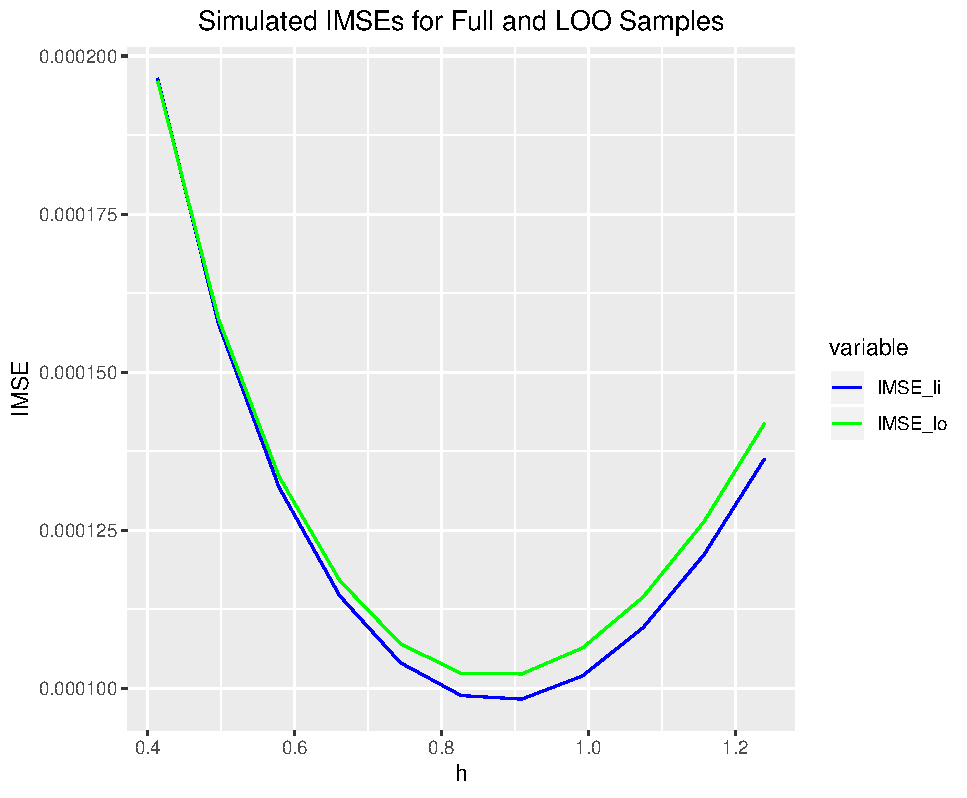
\includegraphics[width=0.8\textwidth]{Q1_IMSE.pdf}
        \caption{Estimated IMSE for $M=1000$ simulations.}

\end{figure}

\textbf{(c)} Somewhat strangely, I find that $h_{\widehat{IMSE,LI}}=h_{\widehat{IMSE,LO}} = 1.1 \times h^*$. I suppose as we increase $M$, the estimates should converge to $h^*$.\\

\textbf{(d)} I get the following rule-of-thumb bandwidth
\begin{align*}
\bar{h}_{\texttt{AIMSE}} = \frac{1}{M} \sum_{i=1}^M \hat{h}_{\texttt{AIMSE},m} \approx 0.985,
\end{align*}
which is about $1.2 \times h^*$.

\newpage

\section{Linear smoothers, cross-validation and series}

\subsection{Local polynomial and series estimation as linear smoothers} We are interested in estimating the regression function $e(x) = \E[y_i | x_i = x]$. The idea of local polynomial regression is to approximate $e(x)$ locally by a polynomial of degree $p$, and estimate this local approximation by weighted least squares. For each $x$ we solve
\begin{align*}
\hat{\mtx{\beta}}(x) &= \arg \min_{\beta \in \R^{p+1}}\sum_{i=1}^n[y_i - \beta_0 - \beta_1(x_i-x) - \beta_2(x_i-x)^2 -...-\beta_p(x_i-x)^p]^2K\left(\frac{x_i - x}{h}\right).
\end{align*}
where
\begin{align*}
\hat e(x) = \hat \beta_0
\end{align*}
Note that this is motivated by a Taylor expansion of the true regression function $e(x_i)$ around $x$. And note that the kernel is just a `smooth' way of weighting observations that are close to the evaluation point $x$.\\

More compactly, we write
\begin{align*}
\hat{\mtx{\beta}}_{\texttt{LP}}(x)  = \arg \min_{\beta \in \R^{p+1}}\sum_{i=1}^n [y_i - \mtx{r}_p(x_i - x)'\mtx{\beta}]^2K\left(\frac{x_i - x}{h}\right)
\end{align*}
where $\mtx{r}_p(u)= (1 , u , u^2 ,...,u^p)'$. \\

Since this is just a weighted least squares problem, we know that
\begin{align*}
\hat{\mtx{\beta}}_{\texttt{LP}}(x)  = (\mtx{R}'_p \mtx{W} \mtx{R}_p)^{-1}\mtx{R}'_p \mtx{W} \mtx{y}
\end{align*}
where
\begin{align*}
\mtx{R}_p = 
\begin{bmatrix}
1 & (x_1 - x) & (x_1-x)^2 & \dots& (x_1-x)^p \\
1 & (x_2 - x) & (x_2-x)^2 & \dots &(x_2-x)^p\\
\vdots & \vdots & \dots & \ddots & \vdots \\
1 & (x_n - x) & (x_n-x)^2 & \dots &(x_n-x)^p
\end{bmatrix}
\end{align*}
and $\mtx{W} = \text{diag}\left(K\left(\frac{x_1 - x}{h}\right), K\left(\frac{x_2 - x}{h}\right),..., K\left(\frac{x_n - x}{h}\right) \right)$.\\

Then
\begin{align*}
\hat{\mtx{e}}(x) &= \mtx{e}_1'\hat{\mtx{\beta}}_{\texttt{LP}}(x)  \\
&=\mtx{e}_1'(\mtx{R}'_p \mtx{W} \mtx{R}_p)^{-1}\mtx{R}'_p \mtx{W} \mtx{y}
\end{align*}
where $ \mtx{e}_1$ the first standard basis vector of length $(1+p)$ (i.e. it has a 1 in the first entry and zeros in the remaining $p$ entries). I think in summation form we can write
\begin{align*}
\hat{\mtx{e}}(x) &= \mtx{e}_1' (\sum_{i=1}^n \mtx{r}_p(x_i-x)\mtx{r}_p(x_i-x)' w_i)^{-1}(\sum_{i=1}^n \mtx{r}_p(x_i-x)w_iy_i)
\end{align*}
where $w_i = K\left(\frac{x_i - x}{h}\right)$.\\

Next we consider series estimation of the regression function $e(x)$. A series approximation to $e(x)$ is a global approximation, unlike the local polynomial regression. A series approximation that uses a polynomial basis (c.f. splines) takes the form
\begin{align*}
\hat{\mtx{\beta}}_{\texttt{Series}} = \arg \min_{\beta \in \R^{p+1}} \sum_{i=1}^n (y_i - \mtx{r}_p(x_i)' \mtx{\beta})^2
\end{align*}
where $\mtx{r}_p(x_i) = (1, x_i, x_i^2, ..., x_i^p)$. And
\begin{align*}
\hat e(x) =  \mtx{r}_p(x)'\hat{\mtx{\beta}}_{\texttt{Series}} 
\end{align*} 

Accordingly, we have
\begin{align*}
\hat{\mtx{\beta}}_{\texttt{Series}} = \left(\mtx{R}'_p \mtx{R}_p \right)^{-1} \mtx{R}_p \mtx{y}
\end{align*}
where
\begin{align*}
\mtx{R}_p = 
\begin{bmatrix}
1 & (x_1) & (x_1)^2 & \dots& (x_1)^p \\
1 & (x_2) & (x_2)^2 & \dots &(x_2)^p\\
\vdots & \vdots & \dots & \ddots & \vdots \\
1 & (x_n) & (x_n)^2 & \dots &(x_n)^p
\end{bmatrix}
\end{align*}
And,
\begin{align*}
\hat e(x) =  \mtx{r}_p(x)' \left(\mtx{R}'_p \mtx{R}_p \right)^{-1} \mtx{R}_p \mtx{y},
\end{align*}
which is of the linear smoother form. In summation form
\begin{align*}
\hat e(x) =  \mtx{r}_p(x)' (\sum_{i=1}^n  \mtx{r}_p(x_i) \mtx{r}_p(x_i)')^{-1} (\sum_{i=1}^n  \mtx{r}_p(x_i) y_i).
\end{align*}

\subsection{Cross validation}
The idea of cross-validation is to choose the tuning parameter (e.g. bandwidth, etc.) that minimizes the mean squared leave-one-out error
\begin{align*}
\hat c = \arg \min_c \frac{1}{n} \sum_{i=1}^n (y_i - \hat e_{(i)}(x_i; c))^2
\end{align*}
where $\hat e_{(i)}(x_i)$ is the estimator of the regression function that ``leaves out'' $x_i$.\\ 

From the above results we know that both the local polynomial and series estimators can be written as
\begin{align*}
\hat{\mtx{e}}(x) = \mtx{S}\mtx{y}
\end{align*}
where $\mtx{S}$ is the `smoothing' matrix. Note that for local polynomial and series estimators the smoothing matrix is constant preserving in the sense $\mtx{S}{\mtx{1}} = \mtx{1}$. That is, the rows of \mtx{S} sum to one. In leave-one-out cross validation, we want to use the same smoother with the $i$-th row and column deleted; we also want this to be an $(n -1) \times (n - 1)$ smoother matrix. Accordingly, we must renormalize the rows to sum to one. Let $w_{ij}$ denote the elements of $\mtx{S}$. When we delete the $i$-th column, then the $i$-th row now sums to $1- w_{ii}$. So, we divide by $1- w_{ii}$ to renormalize. Accordingly, the leave-one-out estimator is
\begin{align*}
\hat e_{(i)}(x_i) = \frac{1}{1-w_{ii}} \sum_{j=1,j\neq i}^n w_{ij}y_i
\end{align*}
And note that the full-sample estimator is just
\begin{align*}
\hat e(x_i) = \sum_{j=1}^n w_{ij}y_i.
\end{align*}
From the above expression we get
\begin{align*}
\hat e_{(i)}(x_i)(1-w_{ii}) &=\sum_{j=1,j\neq i}^n w_{ij}y_i\\
\hat e_{(i)}(x_i) &= \sum_{j=1,j\neq i}^n w_{ij}y_i + w_{ii}\hat e_{(i)}(x_i)\\
&=\sum_{j=1}^n w_{ij}y_i + w_{ii}\hat e_{(i)}(x_i) - w_{ii}y_i\\
&=\hat e(x_i)  + w_{ii}\hat e_{(i)}(x_i) - w_{ii}y_i\\
\implies y_i - \hat e_{(i)}(x_i) &= y_i -\hat e(x_i)  - w_{ii}\hat e_{(i)}(x_i) + w_{ii}y_i\\
&=y_i - \hat e(x_i) + w_{ii}(y_i - \hat e_{(i)}(x_i))\\
\therefore y_i - \hat e_{(i)}(x_i) &= \frac{1}{1-w_{ii}}(y_i - \hat e(x_i)),
\end{align*}
which gives the desired result.

\subsection{Asymptotic distribution}
First note that we have iid data. Also note that we must have $\sum_{i=1}^n w_{n,i}(x_i) = 1$. To ease notation, denote $\E[\cdot | x_1, x_2,...,x_n; x]$ as $\E[\cdot| x]$. Then
\begin{align*}
\E[\hat e(x)|x] &= \E[\sum_{i=1}^n w_{n,i}(x_i)y_i|x]\\
&=\sum_{i=1}^n\E[ w_{n,i}(x_i)y_i|x]\\
&=\sum_{i=1}^nw_{n,i}(x_i)\E[y_i|x]\\
&=\E[y_i|x].
\end{align*}
Thus, so long as $\hat e(x)$ has a finite second moment we can use the classical CLT to get asymptotic normality. Now, 
\begin{align*}
\V[\hat e(x) | x] &= \V[\sum_{i=1}^n w_{n,i}(x)y_i|x]\\
&=\sum_{i=1}^n\V[w_{n,i}(x)y_i|x]\\
&=\V[y_i|x]\sum_{i=1}^nw_{n,i}(x)^2\\
\end{align*}
Then we get the consistent variance estimator
\begin{align*}
\hat{V}(x) = \hat{\sigma}^2  \sum_{i=1}^nw_{n,i}(x)^2
\end{align*}
where $\hat{\sigma}^2 = \frac{1}{n-1}\sum_{i=1}^n (y_i - \hat e(x_i))^2$


\subsection{Confidence intervals}
The pointwise asymptotically valid 95\% CI for $e(x)$ is
\begin{align*}
CI_{95}(x) = [ \hat e(x) - 1.96 \sqrt{\hat{V}(x)},\hat e(x) + 1.96\cdot \sqrt{\hat{V}(x)}].
\end{align*}
This is clearly different to a confidence band that is uniformly valid over all $x$. Uniform confidence bands would be specified as
 \begin{align*}
\sup_{x \in \chi}\left|\frac{\hat e(x) - e(x)}{\sqrt{\hat\V(x)}} \right| \leq q_{1-\alpha/2},
\end{align*}
which is clearly a harder problem than the pointwise intervals.

\subsection{Monte Carlo experiment}

\textbf{(a)} See attached code.\\

\textbf{(b)} I plot the average CV(K), across the $M=1000$ simulations below. 

\begin{figure}[h!]
    \centering
    
        %\centering
        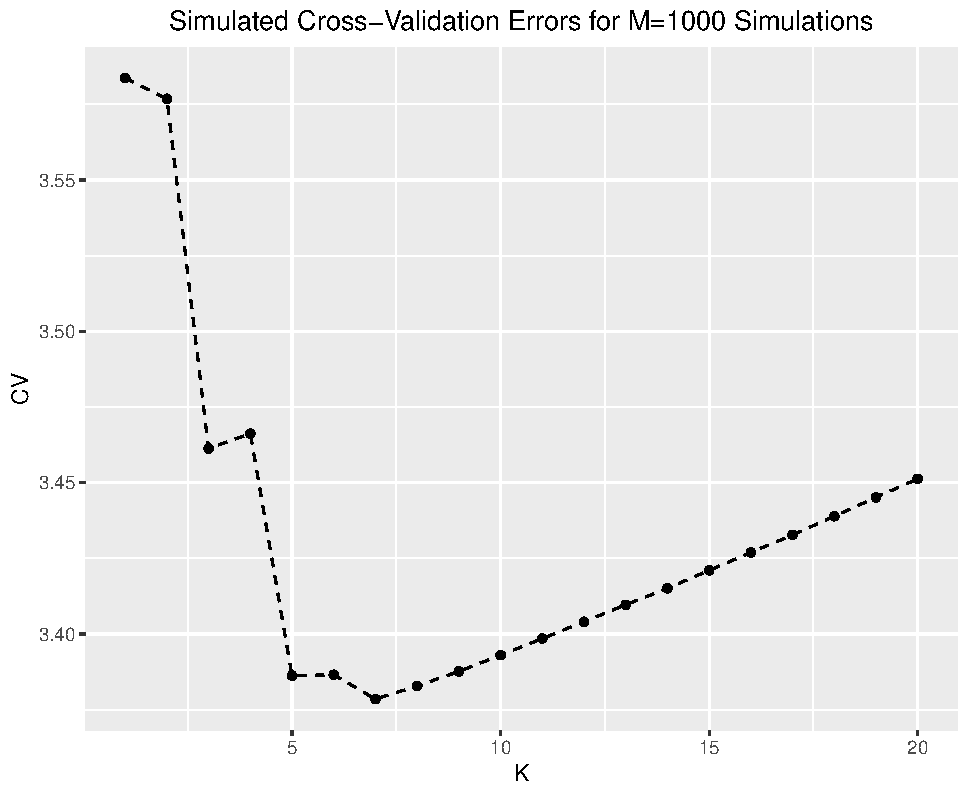
\includegraphics[width=0.7\textwidth]{Q2_CV.pdf}
        \caption{Estimated CV error for $M=1000$ simulations.}

\end{figure}
\newpage

Accordingly, the cross validation polynomial order is $\hat K_{CV} = 7 $.\\

\textbf{(c)} I plot the true regression function and the series estimate below.

\begin{figure}[h!]
    \centering
    
        %\centering
        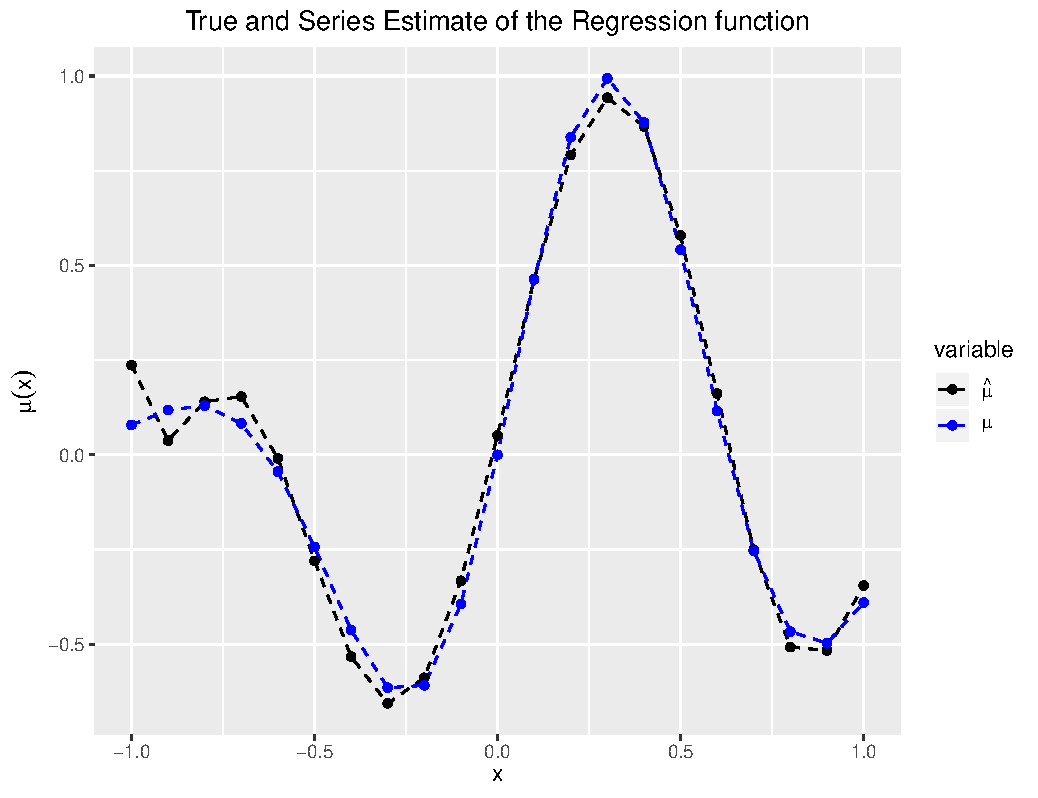
\includegraphics[width=0.7\textwidth]{Q2_diag.pdf}
        %\caption{}
\end{figure}

\textbf{(d)} Next we want to estimate the derivative of the true regression function. I shall assume that $\hat K_{CV}=7$ is also the optimal order for the series estimate of $\mu^{(1)}(x)$. Now, the derivative of the true regression function is
\begin{align*}
\frac{d}{dx}\mu(x) = \exp(-0.1(4x-1)^2)\left[5 \cos(5x) - 0.8 (4x-1)\sin(5x)\right].
\end{align*}
And the series estimate of the derivative is simply the derivative of the original series estimate:
\begin{align*}
\widehat{\frac{d}{dx}\mu(x)}&=\frac{d}{dx}\hat \mu(x)\\
&=(0,1,2x,3x^2,4x^3,5x^4,6x^5,7x^6) \cdot \hat{\beta}_{CV}
\end{align*}
I plot the true derivative and the series estimate below.

\begin{figure}[h!]
    \centering
    
        %\centering
        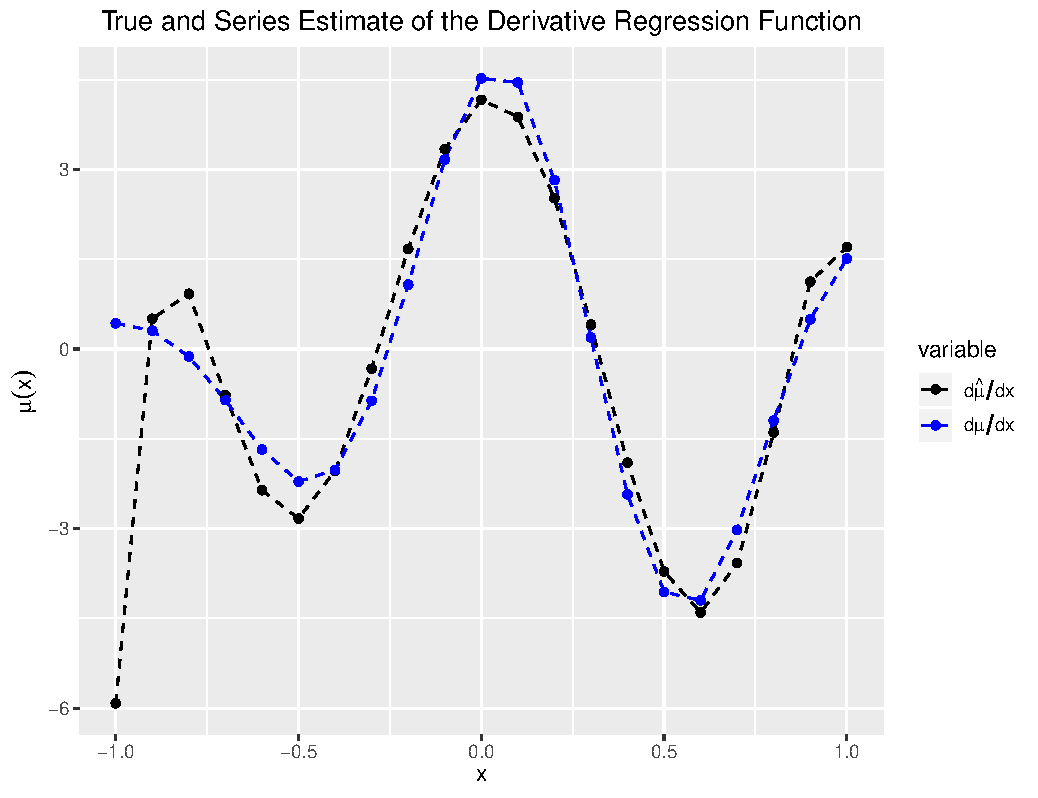
\includegraphics[width=0.7\textwidth]{Q2_diagder.pdf}
        %\caption{}
\end{figure}



\newpage

\section{Semiparametric semi-linear model}
We have the partially linear model
\begin{align}
y_i = t_i \theta_0 + g_0(\mtx{x_i}) + \e_i, \label{eq:3a}
\end{align}
with the usual heteroskedasticity assumptions for the error.
\subsection{Identification}
From Li-Racine 7.1.1 (p 222) we know that for $\theta_0$ to be identifiable, $t_i$ must not contain a constant (since $t_i$ is a treatment dummy, this is clearly satisfied) or any deterministic functions of $\mtx{x}_i$. 

Now, somehow we need to show
\begin{align*}
\E[(t_i-h_0(\mtx{x}_i))(y_i - t_i\theta_0)]&=0
\end{align*}
Then we have
\begin{align*}
\E[y_i (t_i-h_0(\mtx{x}_i))- t_i\theta_0(t_i-h_0(\mtx{x}_i))]&=0\\
\E[t_i\theta_0(t_i-h_0(\mtx{x}_i))] &= \E[y_i (t_i-h_0(\mtx{x}_i))]\\
\therefore \theta_0 &= \E[t_i(t_i-h_0(\mtx{x}_i))]^{-1}\E[y_i (t_i-h_0(\mtx{x}_i))].
\end{align*}
The IV interpretation is that we are using $t_i-h_0(\mtx{x}_i)$ as an instrument for $t_i$.

\subsection{Series estimation}
\textbf{(a)} Consider the power series approximation
\begin{align*}
\E[y_i |\mtx{x}_i] \approx t_i \theta_0 + \mtx{p}^K(\mtx{x}_i)'\mtx{\gamma}_K.
\end{align*}
Using the usual partition regression formula we get the OLS estimator
\begin{align*}
\hat \theta(K) = (\mtx{t}'\mtx{M}_{P}\mtx{t})^{-1}\mtx{t}'\mtx{M}_P\mtx{y}
\end{align*}
where $\mtx{t} = (t_1, ...,t_n)'$ and 
\begin{align*}
\mtx{M}_P = \mtx{I} - \mtx{P}_{r_p(x)}
\end{align*}
and
\begin{align*}
\mtx{P}_{r_p(x)} =\mtx{R}_p \left(\mtx{R}'_p \mtx{R}_p \right)^{-1} \mtx{R}'_p \
\end{align*}
\begin{align*}
\mtx{R}_p = 
\begin{bmatrix}
1 & (\mtx{x}_1) & (\mtx{x}_1)^2 & \dots& (\mtx{x}_1)^p \\
1 & (\mtx{x}_2) & (\mtx{x}_2)^2 & \dots& (\mtx{x}_2)^p\\
\vdots & \vdots & \dots & \ddots & \vdots \\
1 & (\mtx{x}_n) & (\mtx{x}_n)^2 & \dots& (\mtx{x}_n)^p
\end{bmatrix}
\end{align*}

\textbf{(b)}
We have the moment condition
\begin{align*}
\theta_0 &= \E[t_i(t_i-h_0(\mtx{x}_i))]^{-1}\E[y_i (t_i-h_0(\mtx{x}_i))]
\end{align*}
The M-estimator is simply
\begin{align*}
\hat \theta_M &=\left(\frac{1}{n}\sum_{i=1}^nt_i(t_i-\hat h(\mtx{x}_i))\right)^{-1} \left(\frac{1}{n}\sum_{i=1}^n y_i (t_i-\hat h(\mtx{x}_i))\right)\\
&=\left(\sum_{i=1}^nt_i(t_i- \hat h(\mtx{x}_i))\right)^{-1} \left(\sum_{i=1}^n y_i (t_i- \hat h(\mtx{x}_i))\right).
\end{align*}
where $\hat h(\mtx{x}_i)$ is the estimated propensity score (could be estimated by logit/probit, etc.)

\subsection{Asymptotics}
For fixed $K$, $\hat \theta(K)$ is just a partition OLS estimator, so standard asymptotic theory is applicable.  \\

\textbf{(a)} The formal justification for the asymptotic normality of $\hat \theta$ follows directly from the partition regression formula above:
\begin{align*}
\hat \theta(K) &= (\mtx{t}'\mtx{M}_{P}\mtx{t})^{-1}\mtx{t}'\mtx{M}_P(\mtx{t}\theta_0 + \mtx{R}_p\mtx{\gamma}_K+ \mtx{e})\\
&=\theta_0 + (\mtx{t}'\mtx{M}_{P}\mtx{t})^{-1}\mtx{t}'\mtx{M}_P\mtx{e}.
\end{align*}
With iid data and conditional heteroskedasticity, we can apply the WLLN and CLT in the usual way to get the desired asymptotic normality result.\\

\textbf{(b)} As usual, the asymptotically valid 95\% CI for $\theta_0$ is
\begin{align*}
CI_{95} = [\hat \theta(K) - 1.96 \sqrt{V_{\texttt{HCO}}},\text{ }\hat \theta(K) + 1.96 \sqrt{V_{\texttt{HCO}}}]
\end{align*}

\newpage

\subsection{Monte Carlo experiment}

\textbf{(a)} See attached code.\\

\textbf{(b)} The table below presents the required statistics computed across the $M=1000$ simulations.

\def\sym#1{\ifmmode^{#1}\else\(^{#1}\)\fi}
\begin{table}[h!]
\caption {\textbf{Simulation Results of Series Estimation of $\theta_0$ in R}}
\centering
\begin{tabular}{l*{5}{r}}
\hline
       $K$     &{$\hat \theta$}&{Bias}&{S.D} & $\hat V_{HCO}$ & Rejection rate\\
\hline
6 & 2.827 & 1.827 & 0.475 & 0.465 & 0.973\\ 
11 & 0.83 & -0.17 & 0.226 & 0.215 & 0.106\\ 
21 & 0.834 & -0.166 & 0.225 & 0.214 & 0.101\\ 
26 & 0.835 & -0.165 & 0.226 & 0.214 & 0.11\\ 
56 & 0.849 & -0.151 & 0.219 & 0.201 & 0.129\\ 
61 & 0.865 & -0.135 & 0.213 & 0.195 & 0.118\\ 
126 & 1.007 & 0.007 & 0.118 & 0.101 & 0.106\\ 
131 & 1.007 & 0.007 & 0.119 & 0.101 & 0.11\\ 
252 & 1.006 & 0.006 & 0.127 & 0.094 & 0.151\\ 
257 & 1.005 & 0.005 & 0.128 & 0.095 & 0.158\\ 
262 & 1.005 & 0.005 & 0.129 & 0.095 & 0.156\\ 
267 & 1.006 & 0.006 & 0.129 & 0.095 & 0.16\\ 
272 & 1.006 & 0.006 & 0.132 & 0.095 & 0.173\\ 
277 & 1.006 & 0.006 & 0.134 & 0.095 & 0.169\\ 


\hline
\multicolumn{6}{ p{10cm} }{\footnotesize \textit{Notes:} column (2,3,5) report the average point estimator, bias and $\hat V_{HCO}$, across the $M$ simulations, respectively; column (4) reports the sample standard deviation of the point estimates; and column (6) reports the proportion of simulations that we would reject $H_0: \theta_0 = 1$.}\\
\end{tabular}
\end{table}

We can clearly see the classic bias/variance trade off: as $K$ increases, bias and variance fall. But as $K$ gets very large, variance of the estimator starts to increase as we're just adding noise.\\

\textbf{(c)} Using cross-validation, I get $\hat K_{CV} = 126$. We can see from Table 1, across the simulations, $\hat K_{CV}$ gives a very low rejection rate; but there are other estimators with lower bias and variance.


\newpage

\section{Appendix: \texttt{R} and \texttt{STATA} code}

\subsection{\texttt{R} code}
\subsubsection{Question 1}


\scriptsize


\begin{verbatim}
## ECON675: ASSIGNMENT 1
## Q3: ANALYSIS OF EXPERIMENTS
## Anirudh Yadav 
## 8/16/2018

######################################################################
# Load packages, clear workspace
######################################################################
rm(list = ls())             #clear workspace
library(dplyr)              #for data manipulation
library(ggplot2)            #for pretty plots
library(boot)               #for bootstrapping
options(scipen = 999)       #forces R to use normal numbers instead of scientific notation


######################################################################
# Input data
######################################################################

# Get LaLonde data
data <- read.csv('PhD_Coursework/ECON675/HW1/LaLonde_1986.csv')

# Convert to data frame
data <- as.data.frame(data)

######################################################################
# Q1 (a): difference in means estimator
######################################################################

# Rename variables
Y.obs       = data$earn78
treat       = data$treat

# Compute difference in means estimator
T.obs.dm    = mean(Y.obs[treat==1],na.rm=TRUE)-mean(Y.obs[treat==0],na.rm=TRUE)


######################################################################
# Q1 (b): conservative confidence intervals
######################################################################
N1 = sum(treat)
N0 = nrow(data)-N1

# Compute "conservative" standard error
s.1                <- sd(Y.obs[treat==1],na.rm=TRUE)^2
s.0                <- sd(Y.obs[treat==0],na.rm=TRUE)^2
se.conserv         <- sqrt(1/N1*s.1 + 1/N0*s.0)

# Compute lower and upper bounds of the interval and store in vector
CI.lower = T.obs.dm - qnorm(0.975)*se.conserv
CI.upper = T.obs.dm + qnorm(0.975)*se.conserv

# Store results
results            <- cbind(T.obs.dm,se.conserv,CI.lower,CI.upper)


######################################################################
# Q2 (a): Fisher Exact P-values
######################################################################

# The FEP function computes Fisher (approximate) p-values for 
# sharp null of no treatment effect, for the difference in means statistic
# and the K-S statistic.

# NOTES: 
# This function takes ~150 secs to run using the KS statistic with 250k draws!
# Is there a more efficient way to do this?


FEP <- function(K=249999,ks=FALSE){
  
  # Initialze vector of length K
  T.vec = vector(length=K)
  
  # Generate K random draws of the assignment vector
  T.MAT = replicate(K,sample(treat))
  
  if(!ks){
  
  # Compute observed difference in means
  T.obs    = mean(Y.obs[treat==1],na.rm=TRUE)-mean(Y.obs[treat==0],na.rm=TRUE)
  
      # Loop through random draws of the assignment vector, 
      # compute and store the test statistic
      for (i in 1:K) {
              T.dm    = mean(Y.obs[T.MAT[,i]==1],na.rm=TRUE)-mean(Y.obs[T.MAT[,i]==0],na.rm=TRUE)
              T.vec[i]            <- T.dm
            }
  
      }else{
    
    # USE K-S statistic
    options(warn=-1) #turn warnings off
    
    # Compute observed KS statistic
    T.obs               <- ks.test(Y.obs[treat==1],Y.obs[treat==0])$statistic
    
    # Loop through random draws of the assignment vector, 
    # compute and store the test statistic
    for (i in 1:K) {
      T.ks               <- ks.test(Y.obs[T.MAT[,i]==1],Y.obs[T.MAT[,i]==0])$statistic
      T.vec[i]           <- T.ks
    }
    
  }
  
  options(warn=0) #turn warnings back on!
  
  
  # Calculate p-value
  p = 1/K*sum(T.vec>=T.obs)
  
  return(p)
  
}


######################################################################
# Q2 (a): Fisher confidence intervals
######################################################################

## First I follow the approach in Imbens & Rubin, s5.7 ##

FisherInterval <- function(K=9999,C.vec=seq(5000,-1500,-250)){

  # Initialize vector of lenght C.vec
  P.vec = vector(length=length(C.vec))

  # Initialze vector of length K
  T.vec = vector(length=K)

  # Generate K random draws of the assignment vector
  T.MAT = replicate(K,sample(treat))
  
  for (j in 1:length(C.vec)){
    
    # Compute observed difference in means
    T.obs    = abs(mean(Y.obs[treat==1],na.rm=TRUE)-mean(Y.obs[treat==0],na.rm=TRUE)- C.vec[j])
    
    # Compute missing potential outcomes under the null
    Y.1 = ifelse(treat==1,Y.obs,Y.obs+C.vec[j])
    Y.0 = ifelse(treat==1,Y.obs-C.vec[j],Y.obs)

      for (i in 1:K) {
          T.dm    = abs(mean(Y.1[T.MAT[,i]==1],na.rm=TRUE)-mean(Y.0[T.MAT[,i]==0],na.rm=TRUE) - C.vec[j])
          T.vec[i]            <- T.dm
          }
  
    p = 1/K*sum(T.vec>=T.obs)
    P.vec[j] <- p
  }
  return(cbind(C.vec,P.vec))
}

# Run function with 10000 draws
# FisherInterval()


## Another way to compute the CI is using bootstrap ##

  # Compute missing potential outcomes under the null
  Y.1 = ifelse(treat==1,Y.obs,Y.obs+T.obs.dm)
  Y.0 = ifelse(treat==1,Y.obs-T.obs.dm,Y.obs)

  # Specify the statistic that we will compute for different permutations
  T.dm <- function(x, ind) {
      T.k <- mean(Y.1[data$treat[ind]==1]) - mean(Y.0[data$treat[ind]==0])
      return(T.k)
  }
  
  # Run bootstrap
  boot.result  <- boot(data = data, R = 9999, statistic = T.dm, sim = "permutation", stype = "i")
  boot.CI      <- quantile(boot.result$t, c(0.025, 0.975))
  
  # Empirical 95% CI for constant treatment effect = T.obs.dm
  print (boot.CI)

######################################################################
# Q3 (a): Plot power function
######################################################################

PowerFun <- function(x) {
            1 - pnorm(qnorm(0.975)-x/se.conserv) + pnorm(-qnorm(0.975)-x/se.conserv)
            }

# Plot usinging ggplot2
p1   <- ggplot(data.frame(x = c(-5000, 5000)), aes(x = x)) + stat_function(fun = PowerFun)

# Plot using curve
curve(1 - pnorm(qnorm(0.975)-x/se.conserv) + 
                pnorm(-qnorm(0.975)-x/se.conserv),-5000,5000,xlab="tau",ylab="Power")


######################################################################
# Q3 (b): Sample size calculation
######################################################################

# Parameterize the equation
p     = 2/3
tau   = 1000

# Write down the power function, which implicitly defines N
# [Note that I use the sample variances to proxy for the population variances]

Fun <- function(N){
        -0.8 + 1 - pnorm(qnorm(0.975)-tau/sqrt(1/N*s.1*(1/p)+1/N*s.0*(1/(1-p)))) +
          pnorm(-qnorm(0.975)-tau/sqrt(1/N*s.1*(1/p)+1/N*s.0*(1/(1-p)))) 
        }

# Solve for N
N.sol <- uniroot(Fun,c(0,100000000))$root
\end{verbatim}

\subsubsection{Question 2}
\begin{verbatim}
## ECON675: ASSIGNMENT 2
## Q1: KERNEL DENSITY ESTIMATION
## Anirudh Yadav 
## 10/7/2018

######################################################################
# Load packages, clear workspace
######################################################################
rm(list = ls())             #clear workspace
library(foreach)
library(dplyr)              #for data manipulation
library(data.table)         #for data manipulation
library(ggplot2)            #for pretty plots
library(boot)               #for bootstrapping
options(scipen = 999)       #forces R to use normal numbers instead of scientific notation



######################################################################
# Q3 (a): compute theoretically optimal bandwidth
######################################################################
# NB. This code only makes sense with the associated tex file...

# Write function to compute second derivative of normal density
d2norm  <- function(x, mu=0, v=1) {
  dnorm(x,mu,sqrt(v))*(((x-mu)/v)^2-1/v)
}

# Second derivative, squared of given Gaussian mixture
myf     <- function(x){
  (0.5*d2norm(x,-1.5,1.5)+0.5*d2norm(x,1,1))^2
}

# Compute required integral
k1     <-integrate(myf, -Inf, Inf)$val

# Compute optimal bandwidth
n      <- 1000
k2     <- 1/5
k3     <- 3/5
P      <- 2

h_aimse <- ((1/(2*P*n))*(factorial(P)/k2)^2*(k3/k1))^(1/(1+2*P))


######################################################################
# Q3 (b): monte carlo
######################################################################

# Function for EP kernel
K.ep    <- function(x){
      y <- .75 * (1-x^2) * (abs(x) <= 1)
      return(y)
}

# Function to compute true density value
f.true  <- function(x){
     y<-0.5*dnorm(x,-1.5,sqrt(1.5))+0.5*dnorm(x,1,1)
     return(y)
}

# Create vector of bandwidths
h.list = h_aimse*seq(0.5,1.5,0.1)

# Generate big matrix of random draws from the given Gaussian DGP
N          <- 1000
M          <- 1000

components <- sample(1:2,prob=c(0.5,0.5),size=n,replace=TRUE)
mu.vec     <- c(-1.5,1)
sd.vec     <- sqrt(c(1.5,1))

set.seed(5290)
X.mat      <- replicate(M,rnorm(n=N,mean=mu.vec[components],sd=sd.vec[components]))

# Function for computing LOO imse for a given bandwidth and random sample
imse.lo         <- function(x.rand=randx, h=h_aimse){
  
  # Compute leave-one-out fhats for each x_i
  y   = sapply(1:N,function(i) 1/(1000*h)*sum(K.ep((as.matrix(x.rand)[-i,]-x.rand[i])/h)))
  
  # Convert y to data.table for easy manipulation
  y   = as.data.table(y)
  
  # Add true density values
  y[, y.true := f.true(x.rand)]
  
  # Compute squared errors
  y[, sq_er.lo := (y - y.true)^2]
  
  # Compute imse.lo
  imse.lo <- y[, mean(sq_er.lo)]
  
  output <- imse.lo
  
  return(output)
}  

# Function for computing full-sample imse for a given bandwidth and random sample
imse.li         <- function(x.rand, h=h_aimse){
  
  # First compute vector of density estimates at each x_i
  y   = sapply(x.rand,function(x) 1/(1000*h)*sum(K.ep((x.rand-x)/h)))
  
  # Convert y to data.table for easy manipulation
  y   = as.data.table(y)
  
  # Add true density values
  y[, y.true := f.true(x.rand)]
  
  # Compute squared errors
  y[, sq_er.li := (y - y.true)^2]
  
  # Compute imse.li
  imse.li <- y[, mean(sq_er.li)]
  
  output <- imse.li
  
  return(output)
}  

# RUN SIMULATIONS - TOTAL RUNTIME APPROX 13-15 MINS
# IMSE_LI <- foreach(h=h.list, .combine='cbind') %:%
#   foreach(i=1:1000, .combine='c') %do% {
#     imse.li(X.mat[,i],h)
#   }
# 
# IMSE_LO <- foreach(h=h.list, .combine='cbind') %:%
#   foreach(i=1:1000, .combine='c') %do% {
#     imse.lo(X.mat[,i],h)
#   }

# Plot IMSEs
# IMSE_comb <- as.data.frame(cbind(h.list,colMeans(IMSE_LI),colMeans(IMSE_LO)))
# colnames(IMSE_comb) <- c("h", "IMSE_li","IMSE_lo")
# g <- melt(IMSE_comb, id="h")
# 
# ggplot(g) + 
#   geom_line(aes(x=h, y=value, colour=variable)) + 
#   scale_colour_manual(values=c("blue","green")) + 
#   labs(title="Simulated IMSEs for Full and LOO Samples",y="IMSE") +theme(plot.title = element_text(hjust = 0.5))


######################################################################
# Q3 (d): rule-of-thumb bandwidth
######################################################################

# Write function to compute squared second derivative of normal density
d2normsq  <- function(x, mu=0, v=1) {
  (dnorm(x,mu,sqrt(v))*(((x-mu)/v)^2-1/v))^2
}


# Write function to compute ROT bandwidth for random sample
h.rot <- function(x.rand){
  
  # Compute sample mean and variance
  mu = mean(x.rand)
  v  = var(x.rand)
  
  # Compute second derivative of normal density
  k1     <-integrate(d2normsq,mu=mu,v=v, -Inf, Inf)$val
  
  # Compute ROT bandwidth
  h <- ((1/N)*(1/k2)^2*(k3/k1))^(1/5)
  
}

# Run simulation using foreach
h.rot.vec <- foreach(i=1:1000, .combine='c') %do% h.rot(X.mat[,i])

# Run simulation using sapply - FASTER!
h.rot.vec2<- sapply(1:M,function(i) h.rot(X.mat[,i]))

# Compute mean h.rot.vec
mean(h.rot.vec2)


\end{verbatim}

\subsubsection{Question 3}

\begin{verbatim}
## ECON675: ASSIGNMENT 2
## Q3: Semiparametric Semi-Linear Model
## Anirudh Yadav 
## 11/10/2018

######################################################################
# Load packages, clear workspace
######################################################################
rm(list = ls())             #clear workspace
library(foreach)            #for looping
library(dplyr)              #for data manipulation
library(data.table)         #for data manipulation
library(ggplot2)            #for pretty plots
library(boot)               #for bootstrapping
library(Matrix)             #fast matrix calcs
options(scipen = 999)       #forces R to use normal numbers instead of scientific notation

######################################################################
# Q4 (a): data generation, ploynomial basis
######################################################################
d   = 5
N   = 500
M   = 1000

DGP    = function(n=N){
    x      = t(as.matrix(replicate(n,runif(d,-1,1))))
    v      = rnorm(n)
    x.norm = sapply(1:n,function(i) t(x[i,])%*%x[i,])
    e      = 0.3637899*(1+x.norm)*v
    g0.x   =exp(x.norm)
    u      = rnorm(n)
    tt     = as.numeric((sqrt(x.norm)+u)>1)
    y      = tt + g0.x + e
 
    return(list(y=y, x=x, tt=tt))
}

# generate the polynomial basis
gen.P = function(Z,K) {
  if (K==0)   out = NULL;
  if (K==1)   out = poly(Z,degree=1,raw=TRUE);
  if (K==2)  {out = poly(Z,degree=1,raw=TRUE); for (j in 1:ncol(Z)) out = cbind(out,Z[,j]^2);}
  if (K==2.5) out = poly(Z,degree=2,raw=TRUE);
  if (K==3)  {out = poly(Z,degree=2,raw=TRUE); for (j in 1:ncol(Z)) out = cbind(out,Z[,j]^3);}
  if (K==3.5) out = poly(Z,degree=3,raw=TRUE);
  if (K==4)  {out = poly(Z,degree=3,raw=TRUE); for (j in 1:ncol(Z)) out = cbind(out,Z[,j]^4);}
  if (K==4.5) out = poly(Z,degree=4,raw=TRUE);
  if (K==5)  {out = poly(Z,degree=4,raw=TRUE); for (j in 1:ncol(Z)) out = cbind(out,Z[,j]^5);}
  if (K==5.5) out = poly(Z,degree=5,raw=TRUE);
  if (K>=6)  {out = poly(Z,degree=5,raw=TRUE); for (k in 6:K) for (j in 1:ncol(Z)) out = cbind(out,Z[,j]^k);}
  ## RETURN POLYNOMIAL BASIS
  return(out)
}

######################################################################
# Q4 (b): monte carlo simulation
######################################################################
K   <- c(1, 2, 2.5, 3, 3.5, 4, 4.5, 5, 5.5, 6, 7, 8, 9, 10)
K.r <- c(6, 11, 21, 26, 56, 61, 126, 131, 252, 257, 262, 267, 272, 277)
nK  <- length(K)
theta.hat <- matrix(NaN, ncol=nK, nrow=M)
se.hat    <- theta.hat


for (m in 1:M) {
  data <- DGP(N)
  X    <- data$x
  Y    <- data$y 
  TT   <- data$tt
  
  for (k in 1:nK) {
    X.pol <- cbind(1, gen.P(X, K[k]))
    X.Q   <- qr.Q(qr(X.pol))
    
    # Compute annihalator matrix
    MP     <- diag(rep(1,N)) - X.Q %*% t(X.Q)
    
    # Pre-multiplly by MP
    Y.M <- MP %*% Y
    TT.M <- MP %*% TT
    
    # Get theta.hat using partition regression
    theta.hat[m, k] <- (t(TT.M) %*% Y.M) / (t(TT.M) %*% TT.M)
    
    # Get standard errors
    Sigma <- diag((as.numeric((Y.M - TT.M*theta.hat[m, k])))^2)
    se.hat[m, k] <- sqrt(t(TT.M) %*% Sigma %*% TT.M) / (t(TT.M) %*% TT.M)
  }
}

# Tabulate results
table <- matrix(NaN, ncol=6, nrow=nK)
for (k in 1:nK) {
  table[k, 1] <- K.r[k]
  table[k, 2] <- mean(theta.hat[, k])                               # point estimate
  table[k, 3] <- mean(theta.hat[, k]) - 1                           # bias
  table[k, 4] <- sd(theta.hat[, k])                                 # standard deviation
  table[k, 5] <- mean(se.hat[, k])                                  # mean standard error
  table[k, 6] <- mean((theta.hat[, k] - 1.96 * se.hat[, k] > 1) | 
                        (theta.hat[, k] + 1.96 * se.hat[, k] < 1))  # rejection rate
}
write.table(round(table,3), "PhD_Coursework/ECON675/HW2/partial_linear.txt", sep=" & ", eol="\\\\ \n", col.names = FALSE, row.names = FALSE)

######################################################################
# Q4 (c): cross-validation
######################################################################

# cross validation function
K.CV <- function(tt, X, Y) {
  temp <- rep(NaN, nK)
  for (k in 1:nK) {
    X.pol <- cbind(1, tt, gen.P(X, K[k]))
    X.Q   <- qr.Q(qr(X.pol))
    XX <- X.Q %*% t(X.Q)
    Y.hat <- XX %*% Y
    W <- diag(XX)
    temp[k] <- mean(((Y-Y.hat) / (1-W))^2)
  }
  return(which.min(temp))
}

theta.hat2 <- rep(NaN, M)
se.hat2    <- theta.hat2
K.hat2     <- theta.hat2



for (m in 1:M) {
  data <- DGP(N)
  X    <- data$x
  Y    <- data$y 
  tt   <- data$tt
  
  k.opt <- K.CV(tt, X, Y)
  K.hat2[m]     <- K.r[k.opt]
}
\end{verbatim}

\newpage

\subsection{\texttt{STATA} code}

\begin{verbatim}
clear all
set more off, perm

global datadir $dir\data
global resdir $dir\results\intermediate

************************************
************ Question 1 ************
************************************

* Some values
global M = 1000 //number of iterations
global n = 1000 
global hvalues .5 .6 .7 .8 0.8199 .9 1 1.1 1.2 1.3 1.4 1.5
mat hvalues = (0.8199, .5, .6, .7, .8, .9, 1, 1.1, 1.2, 1.3, 1.4, 1.5)

*DGP Values
global mu1 = -1.5
global mu2 = 1
global sd1 = sqrt(1.5)
global sd2 = 1
	
	mata:
	//**********FUNCTIONS***********
	// function for calculating kernel 
	real scalar function kern(real scalar u){
		return(.75*(1-u^2)*(abs(u)<=1))
		}
	
	// function for calculating true density
	real scalar function f_true(real scalar u){
		return(.5*normalden(u,-1.5,sqrt(1.5)) + .5*normalden(u,1,1))
		}
		
	// function for calculating MSE (LI & LO)
	real vector function mse(real vector xdata, real scalar hvalue){
		//Construct two matrices of xdata
		M1 = J($n,$n,.) // n x n matrix with one column for each observation
		M2 = J($n,$n,.) // n x n matrix with one row for each observation
		for (i=1; i<= $n; i++) {
			v = J($n,1,xdata[i])
			M1[,i] = v
			M2[i,] = v'
			}
		
		M3 = (M1-M2)/hvalue //object to be evaluated by kernel
		M4 = J($n,$n,.)
		M5 = J($n,$n,.)
		fx = J($n,1,.)
		
		for (i=1; i<=$n; i++){
			for (j=1; j<=$n; j++){
				M4[i,j] = kern(M3[i,j])
			}
			M5[i,] = M4[i,]
			M5[i,i]=0
			
			fx[i,1] = f_true(xdata[i])
		}
		
		fhat_LI = rowsum(M4)/($n*hvalue)
		fhat_LO = rowsum(M5)/(($n-1)*hvalue)
		
		sqe_LI = (fhat_LI-fx):^2
		sqe_LO = (fhat_LO-fx):^2
		
		mse_LI = mean(sqe_LI)
		mse_LO = mean(sqe_LO)
		
		return((mse_LI,mse_LO))
		}
	
	// function for importing/exporting to mata for mse calculation
	void iteration(real scalar m){
		x= st_data(.,.)
		hvalues = st_matrix("hvalues")
		
		mse = J(12,2,.)
		for (h=1; h<=12; h++){
			mse[h,] = mse(x,hvalues[1,h])
		}	
		st_matrix("msetemp",mse)
		}
	end

	
	*Empty matrix to be filled
	mat msesum = J(12,2,0)
	
	*Loop through iterations
	timer on 1
	forval m = 1/$M{
	disp `m'
	set obs $n
	
	*equally weight two normal distributions
	gen comps = uniform() >= .5

	*generate sample 
	gen x = comps*rnormal($mu1,$sd1) + (1-comps)*rnormal($mu2,$sd2)
	drop comps
	
	*call mata function to calculate mse
	mata iteration(`m')
	drop x
	mat msesum = msesum + msetemp
	}
timer off 1
timer list

mat imse = msesum*1000
svmat imse
rename imse1 imse_li
rename imse2 imse_lo

egen h = fill(.5, .6, .7, .8, 0.8199, .9, 1, 1.1, 1.2, 1.3, 1.4, 1.5)

twoway(line imse_li h)(line imse_lo h), ytitle("IMSE (Thousands)") ///
xtitle("h") xline(0.8199) caption("Note: Vertical line is at h_AMSE")
graph export $resdir/pset2q1.png, replace



/*
timer on 1
program IMSEsim, rclass
drop _all
set obs 1000
gen x =  rnormal(-1/4, 5/8)
gen fx = normalden(-1/4, 5/8)
_kdens x, at(x) generate(fxh) bw(.5) kernel(epan2)
gen diffLI = (fx-fxh)^2
gen diffL0 = 0
gen rng = x
forvalues i = 1/1000 {
	replace x = rng
	replace x = . if _n == `i'
	_kdens x, at(rng) generate(fxh`i') bw(.5) kernel(epan2) 
	replace diffL0 = (fx - fxh`i')^2 if _n == `i'
}
qui summ diffLI
return scalar data1 = r(mean)
qui summ diffL0
return scalar data2 = r(mean)
end
set seed 12345
simulate IMSE_LI=r(data1) IMSE_L0 = r(data2), reps(1) nodots: IMSEsim
timer off 1
timer list
/*


********************************************************************************
*** Question 2: Linear Smoothers, Cross-Validation, and Series
********************************************************************************

clear all

********************************************************************************
* Q2.5b
set obs 1000

* mata function to calculate CV statistic
* CV(list, i): list=variable list, i = max polynomial
mata
void CV(list, i) {
st_view(y=., ., "y")
st_view(X=., ., tokens(list))
XpX  = cross(X, X)
XpXinv  = invsym(XpX)
b  = XpXinv*cross(X, y)
w = diagonal(X*XpXinv*X')
muhat = X*b
num = (y - muhat):*(y - muhat)
den= (J(1000,1,1) - w):*(J(1000,1,1) - w)
div = num:/den
CV = mean(div)
CV
st_numscalar("mCV"+strofreal(i), CV)
}
end

* Program which runs the monte-carlo experiment
program CVsim, rclass
drop _all
set obs 1000
forvalues i = 0/20 { 
gen CV`i' = 0
}
gen x = runiform(-1,1)
gen e = x^2*(rchi2(5)-5)
gen y = exp(-0.1*(4*x-1)^2)*sin(5*x)+e
forvalues i = 0/20 {
gen x`i' = x^`i'
}
forvalues i = 0/20 {
	global xlist = "x0-x`i'"
	di "$xlist"
	mata CV("$xlist", `i')
	replace CV`i' = mCV`i'
	}
end 

* Run the experiment
set seed 22
simulate CV0=CV0 CV1=CV1 CV2=CV2 CV3=CV3 CV4=CV4 CV5=CV5 CV6=CV6 CV7=CV7 CV8=CV8 /// 
		 CV9=CV9 CV10=CV10 CV11=CV11 CV12=CV12 CV13=CV13 CV14=CV14 CV15=CV15 ///
		 CV16=CV16 CV17=CV17 CV18=CV18 CV19=CV19 CV20=CV20, reps(100) nodots: CVsim
collapse *
gen i = 1

reshape long CV, i(i) j(k)
sort CV
local min = k[1]
twoway scatter CV k, ytitle("Mean CV") xtitle("K") xlabel(0(2)20) xmtick(0(1)20) xline(`min')

graph export q2_5b_S.png, replace

********************************************************************************
* Q2.5c
* Program which runs the monte-carlo experiment. At the beginning we generate new
* data, then we call the mata command
program muhatsim, rclass
drop _all
set obs 1000
gen x = runiform(-1,1)
gen e = x^2*(rchi2(5)-5)
gen y = exp(-0.1*(4*x-1)^2)*sin(5*x)+e
forvalues p = 0/7 { 
gen x`p' = x^`p'
}
reg y x0-x7, nocons
clear
set obs 11
gen n = _n
gen foo = 1
gen x = -1+(_n-1)/5
forvalues p = 0/7 { 
gen x`p' = x^`p'
}
predict muhat
predict se, stdp
generate lb = muhat - invnormal(0.975)*se
generate ub = muhat + invnormal(0.975)*se
// gen muhat = _b[x0]*xgp0 + _b[x1]*xgp1 + _b[x2]*xgp2+ _b[x3]*xgp3 + _b[x4]*xgp4	///
//			+ _b[x5]*xgp5 + _b[x6]*xgp6 + _b[x7]*xgp7
keep n muhat foo lb ub 
reshape wide muhat lb ub, i(foo) j(n)
end
set seed 22
simulate muhat1=muhat1 muhat2=muhat2 muhat3=muhat3 muhat4=muhat4 muhat5=muhat5 ///
	muhat6=muhat6 muhat7=muhat7 muhat8=muhat8 muhat9=muhat9 muhat10=muhat10 muhat11=muhat11 ///
	ub1=ub1 ub2=ub2 ub3=ub3 ub4=ub4 ub5=ub5 ub6=ub6 ub7=ub7 ub8=ub8 ub9=ub9 ub10=ub10 ub11=ub11 ///
	lb1=lb1 lb2=lb2 lb3=lb3 lb4=lb4 lb5=lb5 lb6=lb6 lb7=lb7 lb8=lb8 lb9=lb9 lb10=lb10 lb11=lb11, reps(1000) nodots: muhatsim
gen i = _n
reshape long muhat ub lb, i(i) j(grid)
collapse muhat ub lb, by(grid)
gen x = -1+ (grid-1)/5
twoway (function y = exp(-0.1*(4*x-1)^2)*sin(5*x), range(-1 1) lcolor(red)) ///
		(line muhat x, lcolor(gs6)) (line lb x, lcolor(gs6) lpattern(dash)) (line ub x, lcolor(gs6) lpattern(dash)), ///
		legend(order(1 "True f" 2 "Estimated f" 3 "Confidence Interval") rows(1)) ytitle(Y) xtitle(X)
graph export q2_5c_S.png, replace
\end{verbatim}

\end{document}
